\documentclass{article}

\usepackage[utf8]{inputenc}
\usepackage{amsmath}
\usepackage{graphicx}
\usepackage{geometry}
\usepackage{float}
\usepackage{hyperref}

% Adjust the page margins
\geometry{a4paper, margin=1in}

\begin{document}

\begin{titlepage}
    \centering
    % Title centered in the middle of the page
    \vspace*{9cm} % Adjust the vertical space for title placement
    {\Huge \textbf{Population Density Insights for Sindh}\par}
    \vspace{0.5cm}
    % Subtitle
    {\Large Findings from the Pakistan Census 2023\par}
    
    % Author and Date at the bottom center
    \vfill
    {\Large Muhammad Azeem Haider\par}
    \vspace{0.5cm}
    {\Large \today\par}
\end{titlepage}

\section*{Introduction}
This document presents an analysis of Sindh's population across its districts, based on data from the Pakistan Census 2023, which provides insights into population, housing, literacy, and other key indicators.

\vspace{0.5cm}

\noindent The analysis addresses two key questions:

\begin{enumerate}
    \item Comparison of land and population ratios across Sindh's districts.
    \item Identification of districts where the average household size exceeds the provincial average.
\end{enumerate}

\noindent According to a United Nations report, the global population is expected to reach approximately 9.7 billion by 2050, with a further increase to 11.2 billion by 2100. Pakistan is projected to be one of the most populous countries, ranking fourth after India, China, and the United States.

\begin{figure}[H]
    \centering
    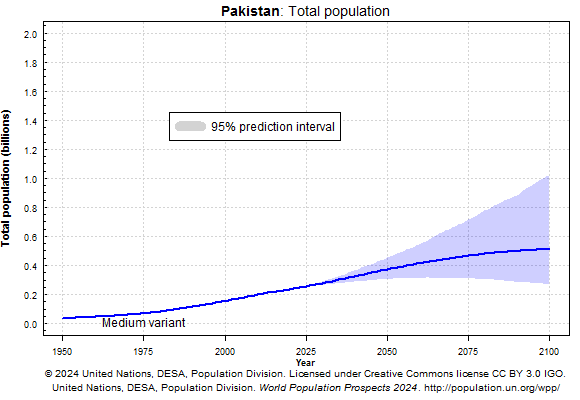
\includegraphics[width=\textwidth]{../Figures/Figure01.png}
    \caption{Projected population growth of Pakistan according to the United Nations.}
    \label{fig:fig1}
\end{figure}

\noindent Figure \ref{fig:fig1} illustrates the projected population growth of Pakistan, which will impact population distribution across its provinces. The information is prediction carried out by the Population Division of the Department of Economic and Social Affairs of the United Nations Secretariat \cite{bib01}.

\vspace{0.5cm}

\noindent The 2023 population census provides valuable information on this distribution. The report from the Pakistan census of 2023 is used as a guiding source \cite{bib02}. The data is analyzed to understand the population distribution across Sindh's districts and identify areas with higher population densities.

\begin{center}
    \begin{tabular}{ |p{3cm}|p{3cm}|p{3cm}|p{3cm}|p{3cm}|  }
        \hline
        \multicolumn{5}{|c|}{Percentage Population Distribution in Different Provinces of Pakistan in Census 2023} \\ 
        \hline
        Balochistan & Sindh & Punjab & Khyber Pakhtunkhwa & Islamabad \\ 
        \hline
        6.2\% & 23.1\% & 52.9\% & 16.9\% & 1.0\% \\ 
        \hline
    \end{tabular}
\end{center}

\noindent Table above shows the percentage distribution of the population across Pakistan's provinces. Sindh, with 23.1\%, has the second-highest population, and its share has steadily increased since the 1961 census. In contrast, other provinces like Balochistan, Punjab, and Khyber Pakhtunkhwa have either fluctuated or seen declines in their population shares.

\begin{figure}[H]
    \centering
    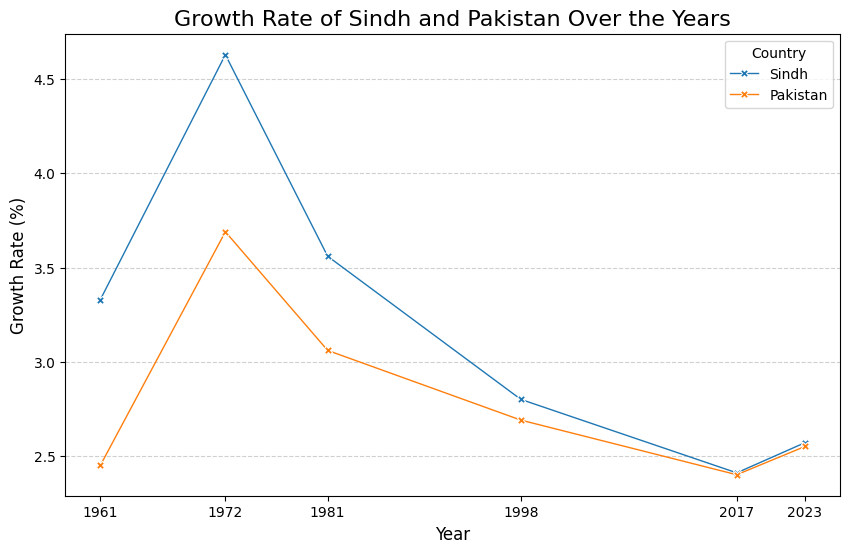
\includegraphics[width=\textwidth]{../Figures/Figure02.png}
    \caption{Population growth trends in Sindh and Pakistan across different censuses.}
    \label{fig:fig2}
\end{figure}

\noindent Figure \ref{fig:fig2} compares the population growth of Sindh and Pakistan across censuses. Historically, Sindh's population growth has been higher than the national average, with the largest gap of 0.94\% observed in 1972. However, this difference has decreased over time, with the 2023 census showing only a 0.02\% difference. This difference was reduced to 0.01\% in the census of 2017. This means that the population growth of Sindh and Pakistan is almost the same since 2017. 

\section*{Analysis}
\noindent Sindh is the second biggest province of Pakistan in terms of population. The province is constantly growing its share of total population in Pakistan. According to the Pakistan census of 2023, Sindh has 30 districts. The land mass of Sindh has 17.70\% of the total land of Pakistan.

% Insert your bibliography style and file here
\bibliographystyle{plain}
\bibliography{references}

\end{document}
